\section{Privacy and Echo Chambers}

To help visualize all the gathered data, identify the presence of echo chambers, and infer the political views of users, super-users' followers were used to create a social network graph and a cosine similarity matrix.

\subsection{Data Preparation}

First, a list of super-users' followers was gathered via TikTok's APIs in the form of a JSON file, and then processed with a script to get the following structure (we can ignore \verb+"videoID"+ and \verb+"videoDate"+):

\begin{lstlisting}[language=json]
[
    {
        "influencer": "ith-super-user Name",
        "videoID": "videoID",
        "videoDate": "videoDate",
        "followerList": [
            "follower1",
            "follower2",
            "follower3",
            "follower4",
            "follower5",
            "follower6",
            "follower-k"
        ]
    }
]
\end{lstlisting}

To clarify, here follows a partition of the real JSON data used:

\begin{lstlisting}[language=json]
    {
        "influencer": "huffpost",
        "videoID": "7354208741996186911",
        "videoDate": "2024-04-05 11:46:08",
        "followerList": [
            "mathieucambet",
            "raphclp",
            "jennet153"
        ]
    },
    {
        "influencer": "huffpost",
        "videoID": "7354208741996186911",
        "videoDate": "2024-04-05 20:46:08",
        "followerList": [
            "doodlegolden0",
            "evanroyalaug",
            "cshanebritt",
            "kabed70"
        ]
    },
\end{lstlisting}

JSON data is then imported to \textit{Social\_Graph.r} for analysis:

\begin{lstlisting}[language=R]
data <- fromJSON(paste(readLines("data.json")))

left_influencer_names <-  # vector of strings with left 
                          # super-user names
right_influencer_names <- # vector of strings with right 
                          # super-user names

# data.frame used to calculate all the graphs and tables
full_total <- data.frame(
  influencer = data$influencer,
  followerList = I(data$followerList)
)

full_influencer_names <- union(left_influencer_names, 
                               right_influencer_names)
\end{lstlisting}

Now we have three data structures to work with: two vectors with all super-users' names and a \verb+data.frame+ that stores all super-users and their gathered followers, as shown below:

\aCapo{}
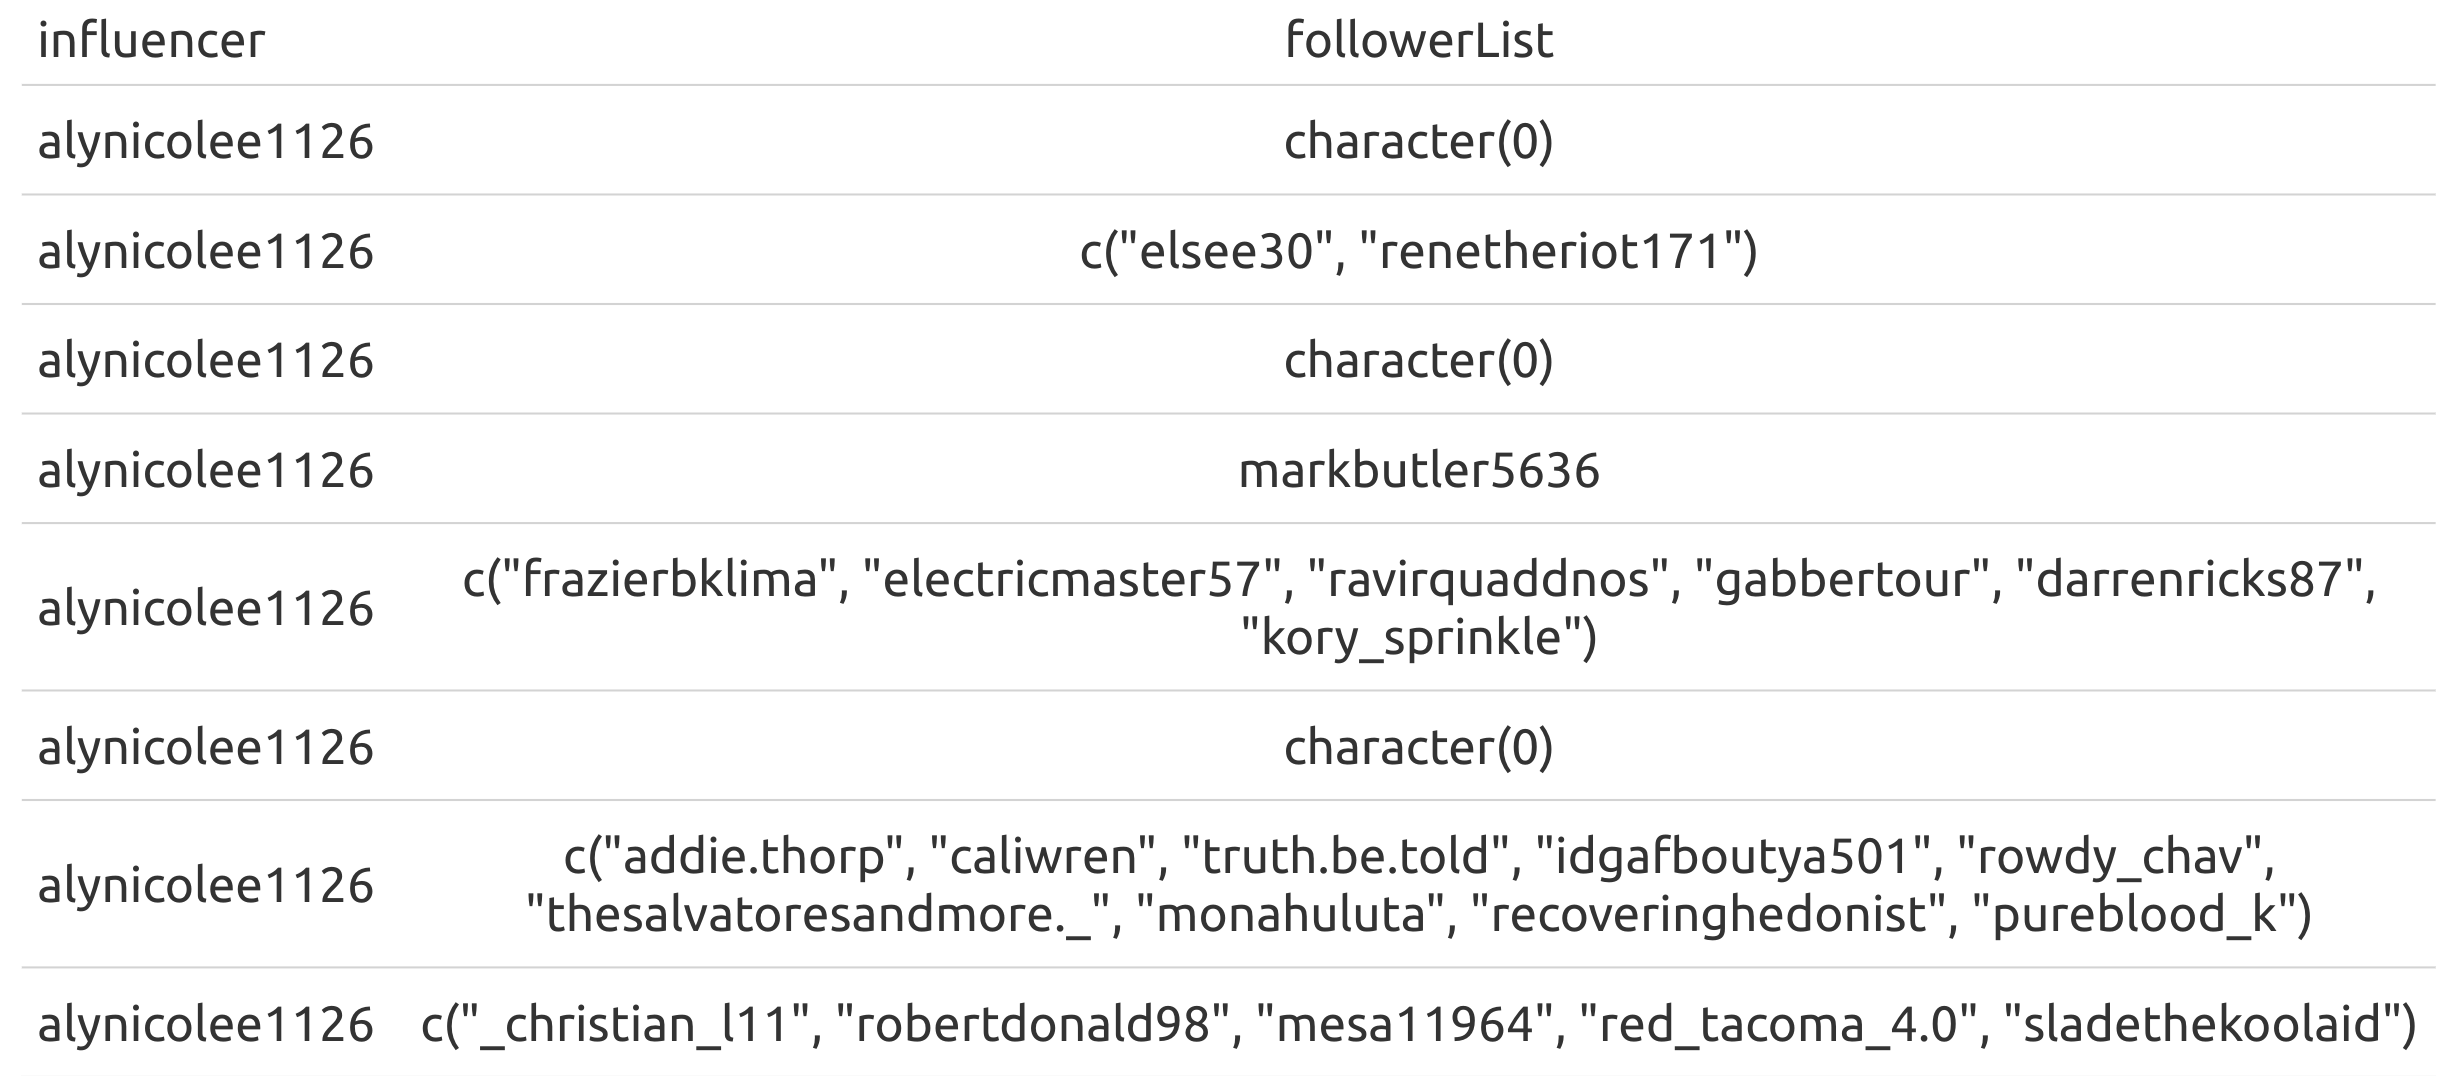
\includegraphics[width = .48\textwidth]{images/total_table_p23.png}

\subsection{Social Graph}

Broadly speaking, a social graph is a graph that represents social relations between entities, were vertices (or nodes) represents users and edges represents relations between such users. It is a model of representation of a social network, and has been referred to as "the global mapping of everybody and how they're related".

To give a brief example: if Alice and Bob are friends on a social network, in a social graph they would be represented each as a node, and there would be an edge between them.

The term was popularized at the Facebook F8 conference on May 24, 2007, when it was used to explain how the newly introduced Facebook Platform would take advantage of the relationships between individuals to offer a richer online experience \cite{wikiSAN}.

\aCapo{}
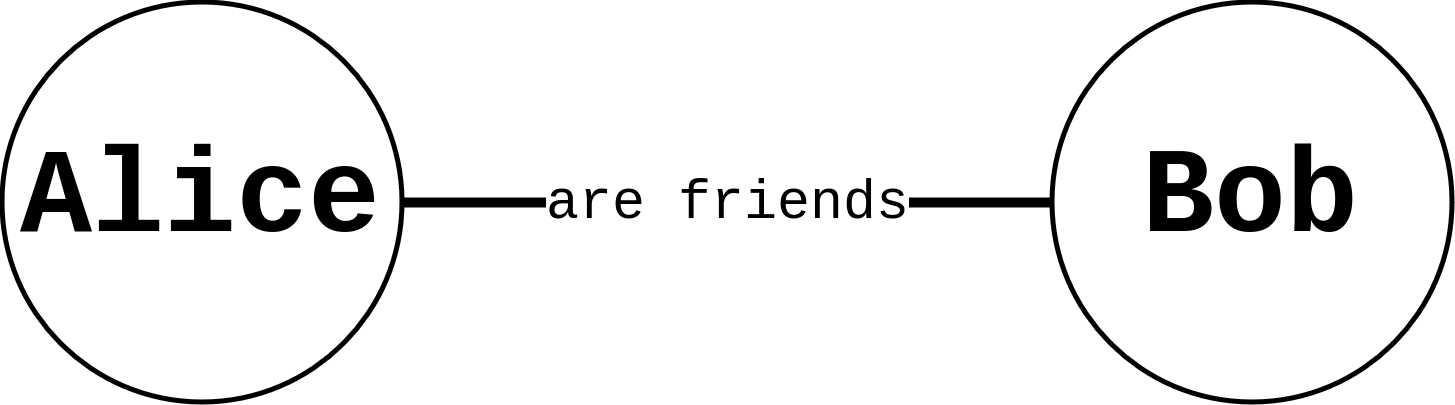
\includegraphics[width = .5\textwidth]{images/alice_bob_san.png}

Employing a social graph has numerous advantages: it helps visualize all gathered data (all users and their relations), identify the presence of echo chambers and provide insights to analyze the network as a whole. \\
The graph that follows clearly demonstrate that, considering the gathered data, users do not interact with each other outside their communities, thus forming cliques that can be interpreted as echo chambers:

\aCapo{}
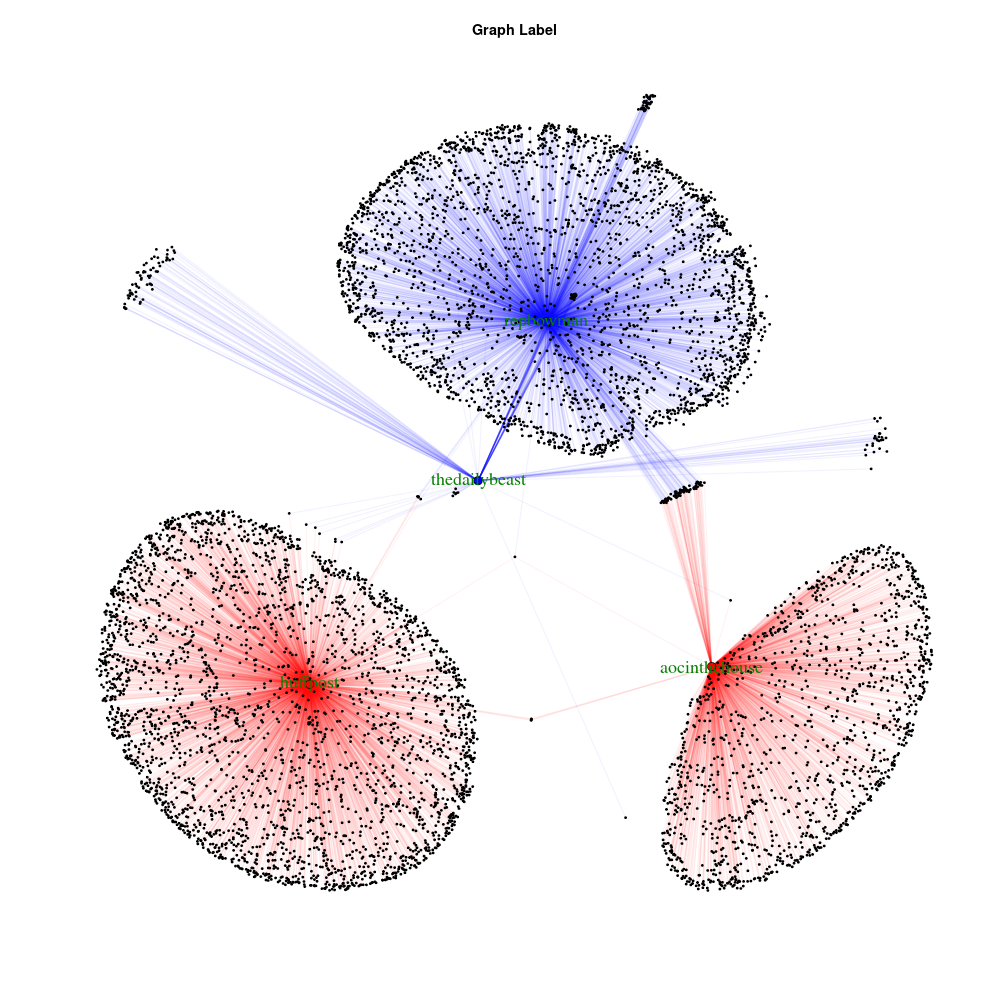
\includegraphics[width = .5\textwidth]{images/mockUP_san.png}

\textcolor{OrangeRed}{The aforementioned graph is actually a mockUp without all the complete data: due to hardware constraints, graph compilation is impossible at the moment of writing (04/06/2024).}

Super-users can be easily identified: their nodes are larger, labeled and, most notably, they are at the center of their respective sub-graphs. 

All black vertices represents followers of the super-users, unlabeled for improved readability, and the edge color represent the political orientation of the super-user they are connected to(red for \textcolor{red}{right-leaning} and blue for \textcolor{blue}{left-leaning} super-users). 

To clarify: if \textit{@user-Alice} follows super-user \textit{@aocinthehouse} (official account of Congress member Alexandria Ocasio-Cortez), which is classified as a left-leaning super-user, the edge connecting them will be blue. 

Conversely, if \textit{@user-Bob} follows super-user \textit{@thesun} (official account of UK's tabloid "The Sun"), which is classified as a right-leaning super-user, the edge connecting them will be red.

\subsection{Cosine Similarity}

Having a graphical representation of a network is valuable: images are easier to recognize, process, and recall. When words enter long-term memory, they do so with a single code. Pictures, on the other hand, contain two codes: one visual and one verbal, each stored in different brain regions (Paivio). The dual-coding nature of images allows two independent ways of accessing visual memories, increasing the odds of remembering at least one. Adding illustrations to text aids comprehension and learning \cite{10.21083/partnership.v10i1.3137}. However, it is also advisable to measure the similarity between users numerically.

Broadly speaking, there are two types of similarity measures between nodes in a network: edge similarity, which provides the index of intersection of parent nodes, and global structure similarity, that aims to evaluate the similarity between two nodes in the context of the whole network. Regarding the latter, Salton Index, Jaccard Index, and Sorensen Index always have good performance, while cosine similarity's computational complexity is very high when applied to large volumes of data \cite{smilarityMeasuresSurvey}. When the data is dense, structure-based indices like Salton's can perform as well as the cosine index but with lower computational complexity. Furthermore, when the data is sparse, structure-based indices outperform the cosine index \cite{10.1016/j.phpro.2010.07.033}.

\aCapo{}
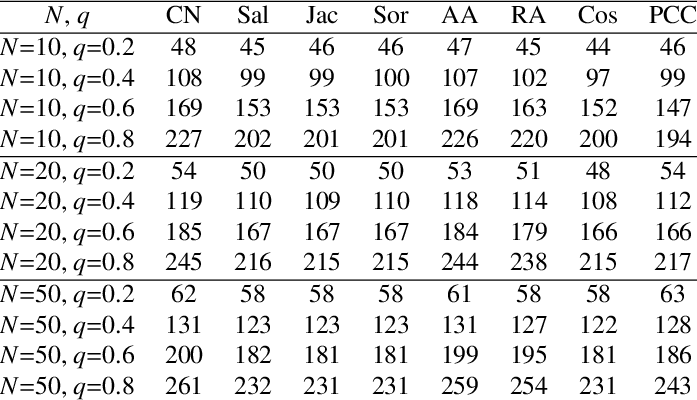
\includegraphics[width = .5\textwidth]{images/salton_precision.png}

The above table shows values regarding precision in inferring similarity between users: Salton index (\textit{Sal} column) seems to perform the best \cite{10.1016/j.phpro.2010.07.033}, therefore it has been used in this work to measure similarity between super-users.

Index formula is as follows: 

$$s_{xy}=\frac{|\Gamma(x)\cap\Gamma(y)|}{\sqrt{k_x\times k_y}}.$$

All index values are calculated for each couple of super-users and shown in the following table where, as mentioned before, blue represent left-leaning and red represent right-leaning super users: 

\aCapo{}
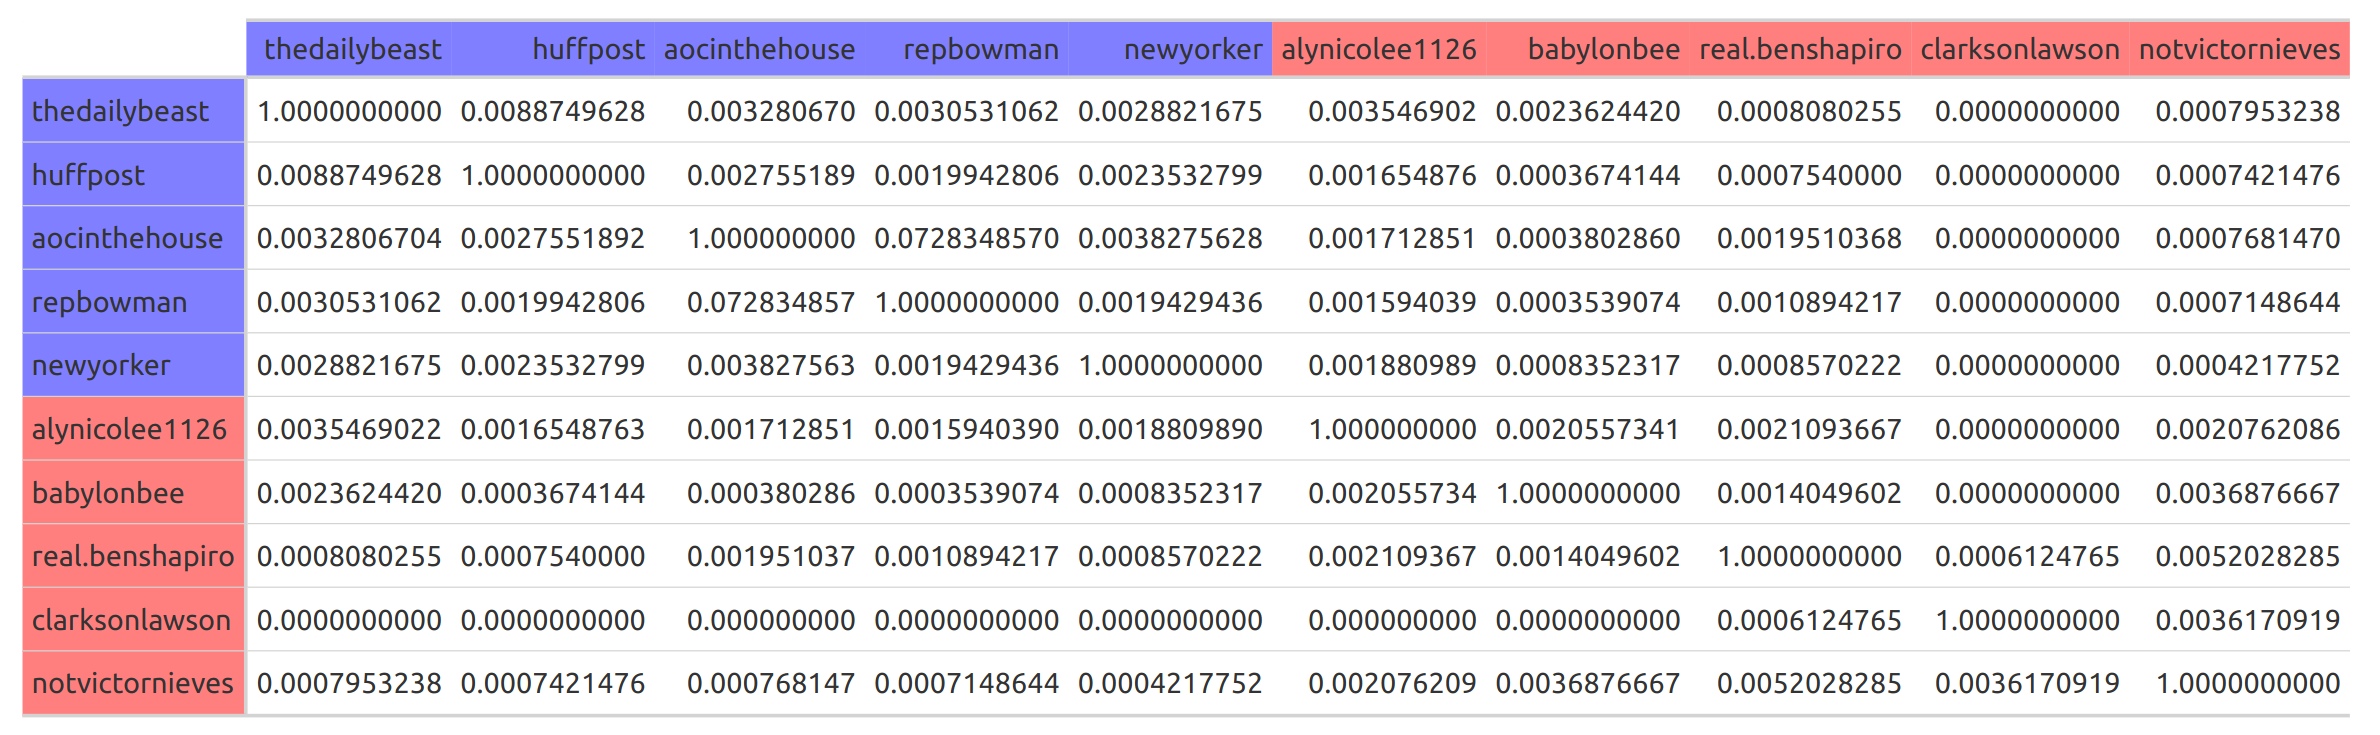
\includegraphics[width = .5\textwidth]{images/final_salton_matrix.png}

Salton index values range between 0 and 1, with the diagonal of the matrix showing all values equal to 1 because a super-user is always identical to itself. The table confirms numerically what could be seen in the social graph: super-users share very few followers, which means that each community is an echo chamber.

\subsection{Privacy Inference}
Another way to leverage social network information, specifically the network structure (edges and their respective nodes), is to infer users' attributes. This falls under classification problems (identifying which of a set of categories an observation belongs to, such as classifying an email as "spam" or "not spam") \cite{wikiClassification}, and such techniques have been employed in this context (e.g., k-nearest neighbors classification \cite{wikiKNN}).

The objective here is to infer the political orientation of users based on the super-users they follow. Given the scarcity of super-users, the presence of only two sets (left and right-leaning), and the high degree of isolation between communities, complex statistical tools are deemed unnecessary. The idea is straightforward: if \textit{user-Alice} follows mainly left-leaning super-users (e.g., \textit{aocinthehouse}, \textit{bernie}, \textit{repbowman}), that user is classified as left-leaning. Conversely, if \textit{user-Bob} follows mainly right-leaning super-users, he is classified as right-leaning.

The following table shows users following more than one super-user from both lists of left and right-leaning super-users, with results ordered by the number of super-users followed.

\aCapo{}
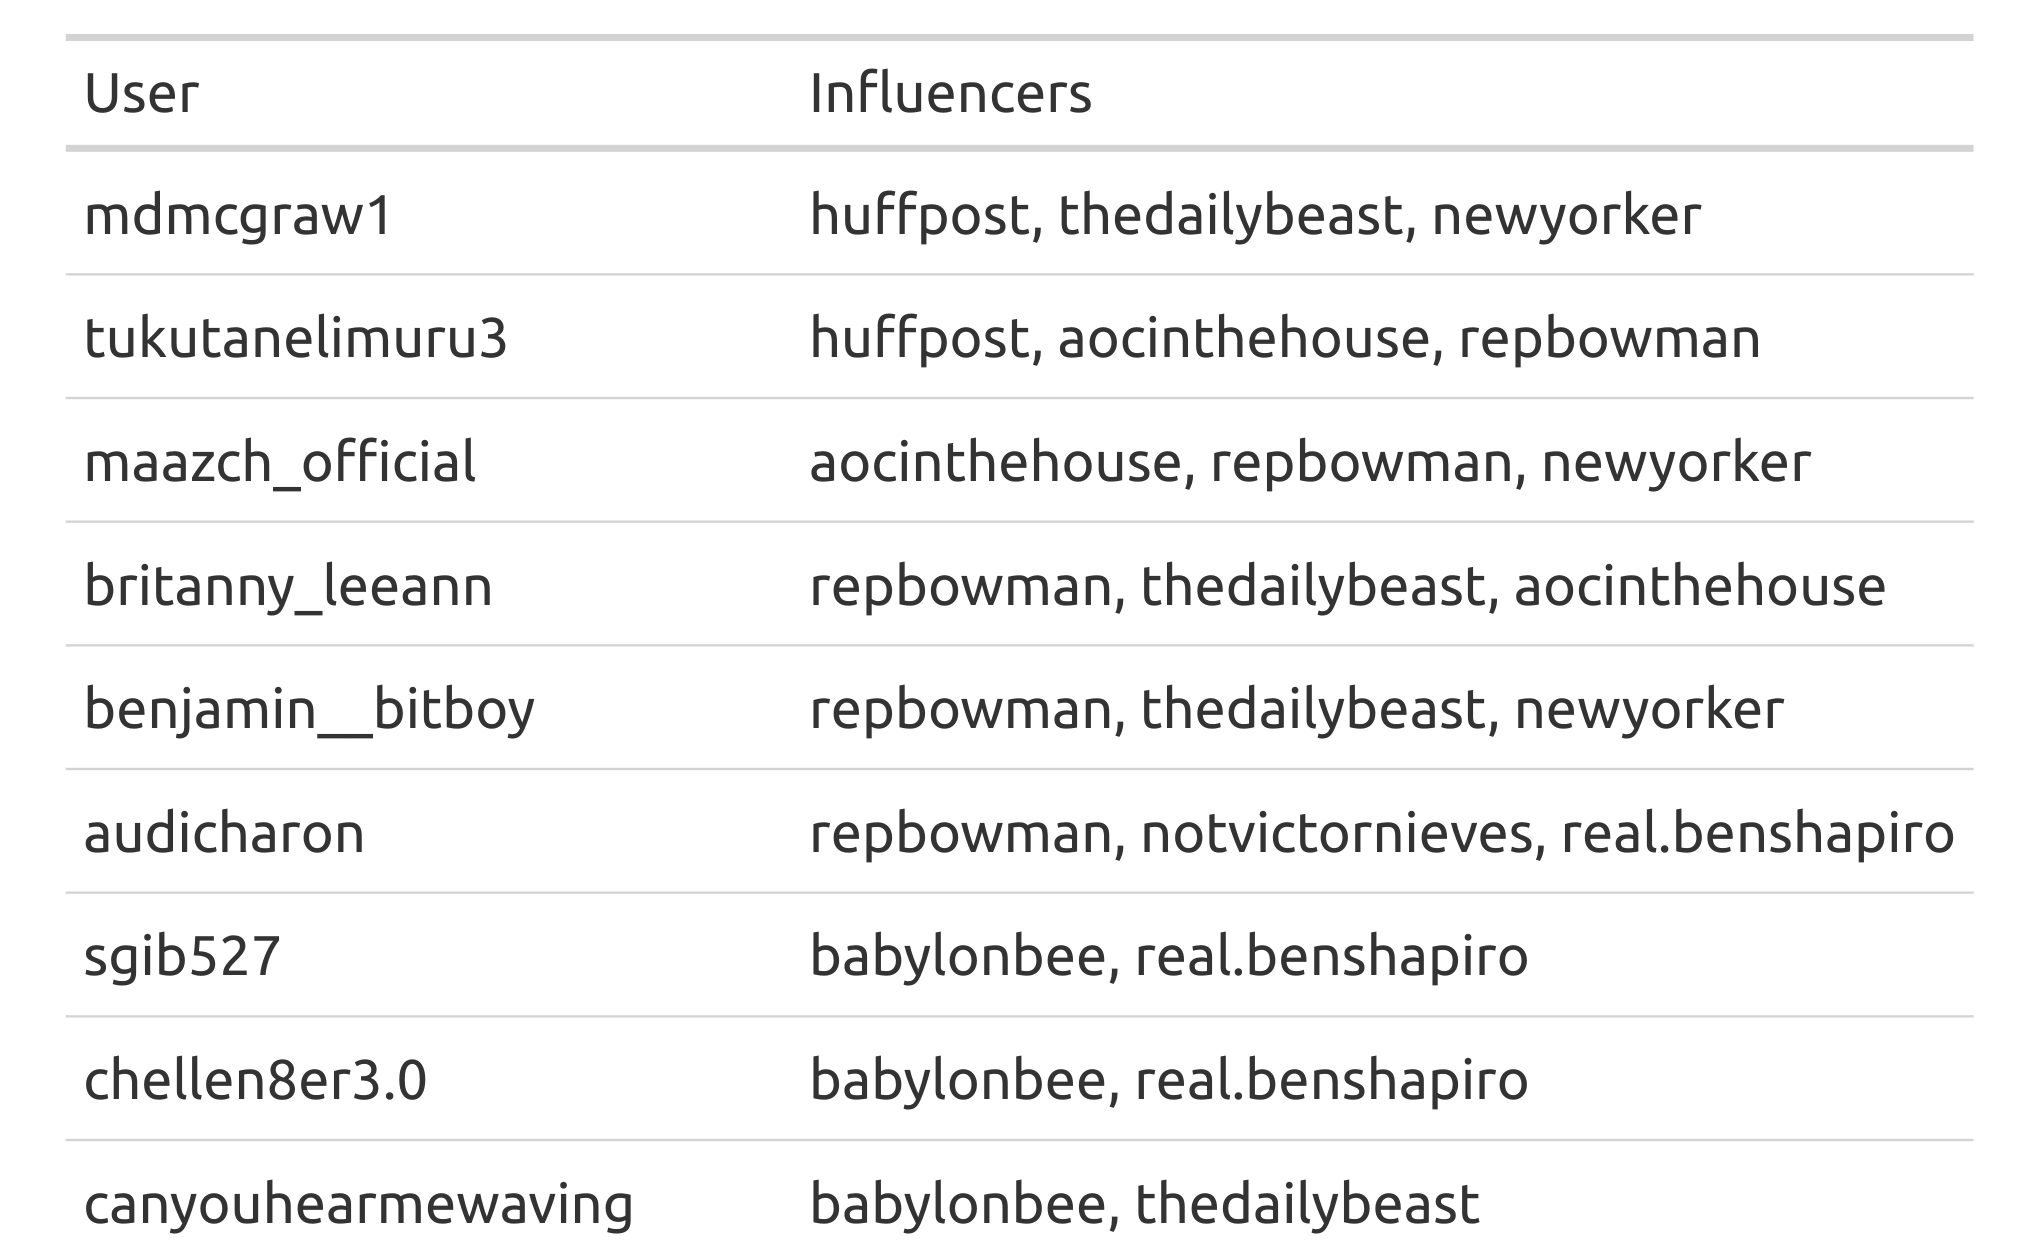
\includegraphics[width = .5\textwidth]{images/final_privacy_table.png}

As we can see, only six users follows more than three super-users and, generally speaking, most users follows super-users of the same political affiliation. Considering the scarcity of data, if a user follows less than 100\% of super-users from the same political spectrum, it is difficult to say anything about their political beliefs.

Let's make some examples: taken into consideration the table shown above (which is a small sample of the original, available a the following link: \url{https://github.com/albertomorini/CNS/blob/main/privacy_table.html}) we can say the following:

\begin{itemize}
    \item User \textit{mdmcgraw1} follows three super-users, all left-leaning, therefore is classified as left-leaning;
    \item User \textit{audicharon} follows three super-users, one left-leaning, two right-leaning, therefore nothing can be said about its political orientation;
    \item User \textit{chellen8er3.0} follows two super-users, both right-leaning, therefore is classified as right-leaning.
\end{itemize}

In future extensions, this classification could be improved by giving weights to super-users: \textit{repbowman} could weight more than \textit{notvictornieves} because the latter is an influencer, while the former is a politician.